\section{Proposed Architecture} \label{architecture}

The current section will describe how the two first goals of
Section~\ref{sec:goals} will be addressed.
Firstly, it presents the chosen approaches in order to build the \emph{Sueca} player (Section \ref{sec:sueca_solution}).
Lastly, it introduces the conceptual model and the architecture of the physical embodied agent that reacts socially according to the game state (Section \ref{sec:social_solution}).


\subsection{\emph{Sueca}}
\label{sec:sueca_solution}

Currently, there are not artificial players of the \emph{Sueca} card game.
Research has shown that the state of the art of imperfect information games is based on Monte Carlo methods.
To build the \emph{Sueca} card game, the chosen approach is similar to what Furtak et. al. have done in the Skat card game.
These two games are identical, excluding the nonexistent bidding phase on \emph{Sueca}.
Furtak et. al. have explored how \gls{pimc}'s results vary according to some of the game's properties and proved its benefits on Skat.
Due to the affinity between the two games, it is predictable that the results of applying \gls{pimc} to \emph{Sueca} are also satisfying.

Furthermore, this \emph{Sueca} player will play against aged people.
Since they are not world champions or are not even at a professional level, the power of the artificial player must be balanced.
On one hand, the idea is to create a challenging environment for the elderly.
On the other hand, an existing concern is not to devastate the self-esteem of them.
The motivation of this work is to create a pleasing and, at the same time, stimulating activity for the elderly.

Additionally, a possible development strategy to follow is \gls{iimc}.
Furtak et. al. shown how this algorithm can improve the results of their Skat player.
Depending on the results of applying \gls{pimc} to our domain, it will be considered a further upgrade to the \emph{Sueca} player.

To reinforce the sampling phase of \gls{pimc}, it will be used an opponent modelling similar to what has been done in Poker.
This model will include cards and actions predictions.
Instead of using the random sampling method of the original \gls{pimc}, cards probabilities will influence the cards sampling in each iteration of the algorithm.
After sampling each world, actions predictions will be used in the simulation of a game to influence the opponents' moves.
This approach aims to introduce some of the common mistakes that the usual player makes, instead of considering always optimal moves.
\todo{Especificar como sera feito? I.e. numero de amostras e procedimento?}


\subsection{The social robot in the game context}
\label{sec:social_solution}

Along with the \emph{Sueca} player, this work aims to develop a robot that is socially present in the environment of the game scenario.
In order to achieve this goal, many concerns arise.
Down below, the model presented in Figure~\ref{fig:model} tries to solve and organise all the components involved.

\begin{figure}[h!]
  \centering
    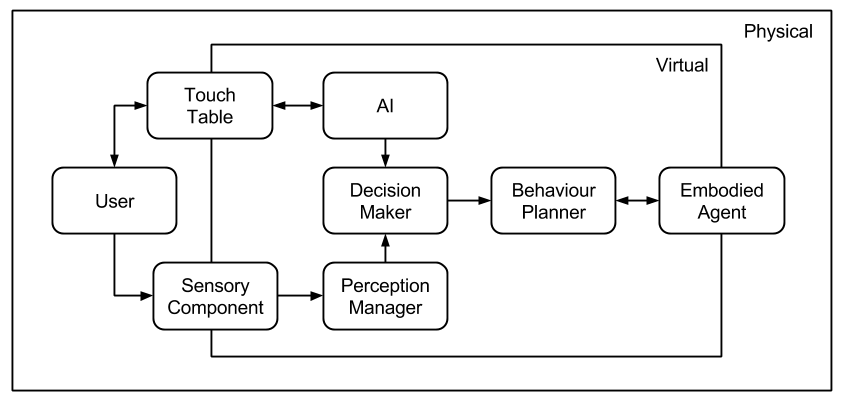
\includegraphics[width=1\textwidth]{./img/model}
  \caption{Structure of the social robot that plays \emph{Sueca}}
\label{fig:model}
\end{figure}

This model distinguishes physical components from virtual ones.
Some entities are not detailed on the scope of this project and are presented as both physical and virtual components.
The human players, Users, will play with physical cards on the top of a Touch Table.
Every game action is detected and communicated to the Game Application.
This module includes all the reasoning about the game and decides the robot actions related to the game.
However, the robot actions also involve social behaviours and this is managed by the Behaviour Planner.
As a result, the Behaviour Planner receives all the sensory input and the game decisions in order to produce an appropriate output and communicate it to the robot.

The architecture that will instantiate the model described above is partially decided.
The virtual layer will be mainly covered by Thalamus framework that allows all the communication between the mentioned entities.
The chosen Behaviour Planner is Skene due to its powerful linkage to the Game Application module.
The Game Application core will be processed offline with the algorithms described in Section~\ref{sec:sueca_solution}.
The robot will initially be \gls{emys} due to its expressiveness.
Nonetheless other robots might be used considering the users' preferences.
Finally, the undecided components are the sensory inputs.
Pereira et. al. have shown the importance of collecting data from user studies.
Theses components will be settled further, after some field research with \emph{Sueca} players.









